\chapter{PENELITIAN TERKAIT}

\section{Sistem Terdistribusi dan Interaksi Layanan Asinkron}
Dalam penelitian ini, sistem terdistribusi dipandang sebagai kumpulan proses yang berkomunikasi untuk menyelesaikan pekerjaan aplikasi. Microservices merupakan salah satu bentuk pengorganisasian aplikasi tersebut: setiap layanan menangani tanggung jawab tertentu. Fokus penelitian bukan kesamaan algoritma pada replika protokol konsensus, melainkan dependensi pekerjaan pada layanan yang berbeda.

Interaksi asinkron dalam proposal ini mencakup pekerjaan yang dapat dilanjutkan dan diselesaikan secara independen sebelum hasilnya digabungkan. Implementasi dapat menggunakan pesan maupun permintaan antarlayanan yang dijalankan secara konkuren. Transportasi HTTP tidak dengan sendirinya membuktikan bahwa aplikasi bersifat sekuensial; sebaliknya, penggunaan antrean juga tidak otomatis menjamin bahwa dependensi bisnis benar. Karena itu, objek yang diperiksa adalah peristiwa bisnis dan hubungan dependensinya.

\section{Happened-Before dan Partial Order}
\label{sec:partial-order}
Misalkan $E$ merupakan himpunan peristiwa. Relasi $\prec$ menyatakan urutan kausal ketat: $a\prec b$ berarti $a$ mendahului $b$ berdasarkan bukti kausal. Relasi dibentuk dari urutan lokal yang benar-benar diketahui, pengiriman dan penerimaan pesan yang bersesuaian, serta penutupan transitifnya \citep{lamport1978}. Dalam graf berarah tanpa siklus, relasi tersebut setara dengan keterjangkauan melalui lintasan berarah yang tidak kosong.

Dua peristiwa disebut tidak terurut dalam observasi apabila tidak ditemukan $a\prec b$ maupun $b\prec a$. Pada model lengkap, pasangan ini dapat dinyatakan konkuren. Pada telemetri yang tidak lengkap, tidak adanya lintasan juga dapat disebabkan oleh bukti yang hilang. Penelitian ini menggunakan istilah tidak terurut ketika kelengkapan belum dapat dijamin, sehingga ketiadaan bukti tidak disamakan dengan kepastian konkurensi.

Urutan total menetapkan posisi bagi setiap pasangan peristiwa. Salah satu urutan total yang mempertahankan semua sisi graf disebut \ist{linear extension} atau urutan topologis. Graf dapat memiliki lebih dari satu urutan topologis. Pada Gambar~\ref{fig:partial-order}, pembayaran dan persediaan memiliki satu asal serta satu penerus bersama, tetapi tidak dipaksa berurutan satu sama lain.

\begin{figure}[H]
  \centering
  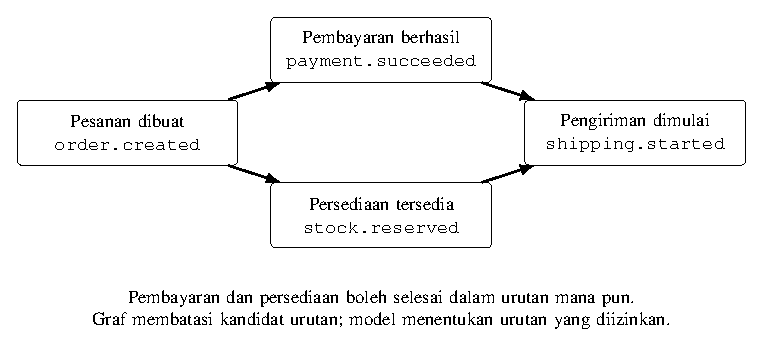
\includegraphics[width=0.95\textwidth]{partial-order}
  \caption{Dependensi bisnis pada alur pemesanan. Timestamp antarlayanan tidak digunakan untuk membentuk sisi graf.}
  \label{fig:partial-order}
\end{figure}

\section{Distributed Tracing dan OpenTelemetry}
\subsection{Trace, Span, dan Peristiwa Bisnis}
Trace mengaitkan span yang merepresentasikan operasi. Span mempunyai identitas, waktu, atribut, dan dapat memuat peristiwa bernama \citep{oteltraces}. Sebuah operasi mempunyai durasi, sedangkan aturan bisnis dapat merujuk pada titik tertentu di dalamnya. Oleh karena itu, penelitian ini memilih unit pemeriksaan berupa titik peristiwa, bukan mengurutkan seluruh durasi span sebagai satu tindakan selesai.

Sebagai ilustrasi, \kode{payment.requested} dan \kode{payment.succeeded} mempunyai arti berbeda. Awal span permintaan tidak membuktikan bahwa transaksi pembayaran telah berhasil. Kontrak yang diusulkan merekam keberhasilan setelah aksi bisnis selesai melalui span event atau span khusus yang dimulai pada titik keberhasilan. Identitas pesanan ditempatkan pada atribut aplikasi agar peristiwa dapat dikelompokkan ke alur kerja yang tepat.

\subsection{Korelasi dan Hubungan Antarsisi Observasi}
Identitas trace dan span digunakan untuk menghubungkan konteks observasi. W3C Trace Context menentukan cara konteks tersebut dibawa lintas komponen \citep{w3ctrace}. Dalam penelitian ini, identitas bisnis seperti \kode{order.id} tetap dibutuhkan: kesamaan trace tidak otomatis sama dengan kesamaan pesanan, dan satu alur kerja dapat mempunyai beberapa konteks trace.

Relasi induk--anak menghubungkan span, sementara link dapat mengaitkan konteks span lain \citep{otelapi}. Penelitian menafsirkan relasi ini pada titik yang dijamin instrumentasi. Awal induk dapat menjadi pendahulu awal anak jika konteks dibuat secara sesuai, tetapi penyelesaian induk atau peristiwa yang dicatat belakangan di induk tidak otomatis mendahului anak. Link umum juga tidak digunakan sebagai jaminan urutan bisnis tanpa kontrak arah yang eksplisit.

Pada komunikasi pesan, konteks pembentukan pesan yang dibawa dari produsen ke konsumen membantu korelasi operasi \citep{otelmessaging}. Pemeriksa masih perlu membedakan satu pesan, beberapa konsumen, dan percobaan pemrosesan ulang. Kesamaan nama operasi atau timestamp tidak cukup untuk mencocokkan pengiriman dengan penerimaan.

\subsection{Kelengkapan Bukti}
Sampling dan batas perekaman dapat memengaruhi bukti yang tersedia \citep{otelsdk}. Penelitian membedakan peristiwa yang hilang dalam aplikasi dari peristiwa yang hilang dalam observasi. Deklarasi kelengkapan hanya boleh berasal dari pengumpulan terkontrol yang mengetahui bahwa semua titik bisnis dan sisi relevan dalam satu alur telah diekspor. Deklarasi tersebut bukan properti yang diperoleh hanya karena semua span mempunyai waktu akhir.

OTLP menyediakan representasi pertukaran data telemetri, termasuk pengodean JSON \citep{otlp}. Format ekspor tidak menetapkan bahwa seluruh fakta bisnis telah diamati. Oleh sebab itu, kesesuaian format dan kelengkapan semantik merupakan dua pemeriksaan yang berbeda.

\section{Semantik Verifikasi Interaksi}
\label{sec:semantik}
Verifikasi runtime memeriksa perilaku yang diamati terhadap spesifikasi. Semantik utama penelitian ini adalah kesesuaian eksistensial: observasi dinyatakan konsisten apabila sedikitnya satu urutan seluruh peristiwa yang mempertahankan hubungan kausal diterima oleh model workflow. Model tersebut berupa state machine kecil yang ditulis pengembang, bukan model formal lengkap implementasi.

Untuk model bahasa $L(P)$ dan graf $G$, kondisi penerimaan ditulis:
\begin{equation}
  \exists\pi\in\operatorname{Lin}(G):\quad \lambda(\pi)\in L(P).
  \label{eq:existential}
\end{equation}
$\operatorname{Lin}(G)$ adalah himpunan urutan topologis graf dan $\lambda$ memetakan peristiwa ke simbol bisnis. Peristiwa konteks yang tidak termasuk alfabet model diproyeksikan keluar dari kata yang diperiksa, tetapi tetap dipertahankan dalam graf agar batasan urutan tidak hilang. Pemetaan ini ditetapkan sebelum evaluasi; peristiwa bisnis yang seharusnya diperiksa tidak boleh diabaikan sebagai konteks.

Sebagai contoh, jika pembayaran dan pengiriman tidak terurut dalam observasi lengkap, urutan pembayaran lalu pengiriman dapat diterima meskipun urutan sebaliknya ditolak. Hasilnya adalah konsisten dengan workflow, bukan bukti bahwa pembayaran benar-benar merupakan pendahulu kausal pengiriman. Jika graf justru menetapkan pengiriman sebelum pembayaran dan model melarang urutan tersebut, tidak ada urutan yang diterima. Apabila graf memiliki beberapa urutan, semuanya memakai model yang sama; tidak cukup memeriksa satu urutan topologis yang kebetulan dipilih.

Semantik ini berbeda dari persyaratan bahwa semua urutan yang kompatibel harus diterima, maupun aturan yang mewajibkan adanya lintasan kausal dari setiap prasyarat menuju tindakan dependen. Kedua persyaratan tersebut tidak menjadi kriteria utama. Konsekuensinya, kesalahan aplikasi yang masih memiliki penjelasan urutan yang diterima tidak selalu dapat dibuktikan dari observasi. Penelitian melaporkan batas ini secara eksplisit.

Pada bukti tidak lengkap, peristiwa atau sisi yang hilang dapat mengubah himpunan urutan dan kata yang diterima. Karena itu, hasil utama keseluruhan workflow memerlukan kontrak kelengkapan; tanpa kontrak tersebut statusnya tidak dapat disimpulkan. Status konsisten hanya berlaku pada model, observasi, dan cakupan workflow yang dinyatakan. Ia bukan pembuktian seluruh implementasi benar atau jaminan liveness pada eksekusi tanpa batas.

\section{Penelitian Terdahulu}
\subsection{Pemeriksaan Kesesuaian pada Microservices}
\citet{sakai2022} membahas pembentukan model proses layanan dari distributed tracing untuk pemeriksaan kesesuaian. Pekerjaan tersebut relevan sebagai contoh pemanfaatan observasi lintas layanan untuk menilai proses. Proposal ini mengambil sumber observasi yang sejenis, tetapi membatasi model pada aturan yang ditulis pengembang dan menelaah semantik dependensi secara eksplisit.

\citet{sun2024} menawarkan pendekatan berbantuan anotasi dan berorientasi skenario untuk mendeteksi inkonsistensi pada sistem microservices. Relevansinya terletak pada pembandingan perilaku aktual dengan ekspektasi aplikasi. Penelitian yang diusulkan tidak mengasumsikan bahwa model aplikasi lengkap dapat diekstraksi secara otomatis; pengembang memberikan sejumlah aturan dan instrumentasi titik bisnis yang dibutuhkan oleh aturan tersebut.

\subsection{Ellsberg dan TraceLink}
Ellsberg menerapkan Runtime Protocol Refinement Checking melalui perbandingan pesan proses dengan eksekusi simulasi protokol, dan mengevaluasinya pada Etcd, ZooKeeper, serta RedisRaft \citep{ding2025}. Objek tersebut berbeda dari alur bisnis antarservice yang menjadi sasaran proposal. Kesamaan terletak pada pemeriksaan bukti eksekusi terhadap perilaku yang diizinkan; spesifikasi dan unit observasinya berbeda.

TraceLink memvalidasi trace implementasi terhadap desain terverifikasi dalam ekosistem PGo, yang menghasilkan TLA+ dan Go dari Modular PlusCal \citep{hackett2025}. Pendekatan tersebut menekankan hubungan antara desain formal dan implementasi serta mempertahankan informasi urutan parsial. Proposal ini tidak menggunakan toolchain PGo atau mengklaim jaminan yang setara; sasaran awalnya adalah aturan aplikasi terbatas pada telemetri OpenTelemetry.

\subsection{Verifikasi Interaksi Menggunakan Automata}
\citet{weilkennedy2025} memeriksa kumpulan trace lokal komunikasi tanpa mengasumsikan jam global bersama dan mengusulkan prosedur berbasis automata. Kajian ini merupakan preprint dan digunakan sebagai pembanding konseptual. Keberadaan prosedur tersebut memperlihatkan bahwa pemeriksaan beberapa urutan yang mungkin bukan kebaruan tersendiri. Proposal ini merancang pencarian urutan topologis yang diterima state machine kecil dari observasi OpenTelemetry. Pemanfaatan automata dan urutan parsial tidak diklaim sebagai kebaruan tersendiri.

\begin{table}[H]
  \centering\small
  \caption{Perbandingan fokus penelitian terkait dan posisi penelitian yang diusulkan}
  \label{tab:related}
  \begin{tabularx}{\textwidth}{@{}p{2.5cm}XX@{}}
    \toprule
    Penelitian & Fokus yang relevan & Perbedaan ruang lingkup proposal \\
    \midrule
    Sakai dan Takahashi & Model proses layanan dari tracing & Workflow eksplisit dari pengembang \\
    Sun dkk. & Inkonsistensi perilaku microservices & Model aturan terbatas, tanpa ekstraksi model lengkap \\
    Ding dkk. & Refinement implementasi protokol & Interaksi aplikasi, bukan protokol konsensus \\
    Hackett dan Beschastnikh & Trace terhadap desain terverifikasi & Kontrak observasi OpenTelemetry, tanpa PGo \\
    Weil-Kennedy dkk. & Interaksi dari trace lokal melalui automata & Ekspor OpenTelemetry dan model workflow terbatas \\
    \bottomrule
  \end{tabularx}
\end{table}

\section{Kesenjangan dan Posisi Penelitian}
Penelitian ditempatkan di antara pemeriksaan proses dari tracing dan validasi trace berbasis spesifikasi formal. Pertanyaan yang diuji adalah apakah kesesuaian urutan workflow yang terbatas dapat diperiksa dari kontrak observasi OpenTelemetry, serta pada kondisi apa hasilnya berbeda dari baseline timestamp. Tiga aspek menjadi perhatian: kecukupan bukti untuk membentuk sisi kausal, pembedaan pelanggaran dari ketidaklengkapan, dan biaya pemeriksaan serta ukuran penjelasan.

Pernyataan kesenjangan ini merupakan posisi penelitian berdasarkan literatur yang telah ditelaah, bukan klaim bahwa seluruh penelitian sebelumnya telah disurvei secara sistematis. Kontribusi yang diharapkan berupa prototipe yang dapat dijalankan, kontrak normalisasi, dataset terkontrol, serta analisis hasil pembandingan. Tidak ditetapkan lebih dahulu bahwa pendekatan kausal selalu lebih unggul; keuntungan, keterbatasan, dan kasus tanpa perbedaan harus dilaporkan.
